Neural networks are widely used across applications like natural language processing~\cite{Transformers} and computer vision~\cite{alexnet, RESNET}. However, their increasing size, often reaching billions of parameters~\cite{Young2017RecentTI,ecoflap}, presents significant computational and memory challenges, making deployment in resource-constrained environments impractical~\cite{ZeRO}. Network pruning has emerged as a key technique to reduce model complexity and enable faster inference~\cite{SparseDNN, PruneFL, snip, GraSP, SynFlow}.

The increase in neural network sizes~\cite{Young2017RecentTI} and the widespread availability of pre-trained models have shifted the focus of pruning strategies. Gradual pruning, which iteratively removes parameters with retraining~\cite{late_training_gupta, Kusupati, gale2019state, RIGL}, is computationally expensive for large models, often requiring days or weeks of fine-tuning~\cite{CHITA}. This becomes infeasible for modern networks, particularly in settings with limited training data, such as privacy-sensitive or low-data scenarios~\cite{WoodFisher}. As a result, one-shot pruning, which compresses pre-trained models in a single step~\cite{WoodFisher, CBS, CHITA, wanda, SparseGPT}, has emerged as a scalable and efficient alternative, directly addressing the runtime and computational cost of gradual pruning for large-scale models.


Pruning methods fall into two categories: \textbf{magnitude pruning (MP)} and \textbf{impact-based pruning (IP)}. MP~\cite{Comparing_Biases, Using_Relevance, hanprune, gordon2020compressing} removes small-magnitude weights, but may not be effective as magnitude alone may not reliably capture parameter importance~\cite{CHITA}. IP methods, such as Optimal Brain Damage~\cite{brain_damage}, Optimal Brain Surgeon~\cite{brain_surgeon}, and their modern extensions, use loss-aware weight selection via second-order approximations to identify and remove low-impact weights, followed by weight updates to compensate for loss. Despite outperforming MP, these methods are computationally expensive as they rely on second-order approximations to select which weights to prune.




This raises an important question:
\textit{What drives the higher pruning quality produced by IP methods compared to MP?}

It is natural to attribute the success of IP methods to \textbf{loss-aware weight selection}, which identifies and preserves critical parameters for the network's performance \cite{brain_damage}. 
\textbf{To test this assumption}, we systematically decouple the two stages of IP: (i) \textbf{weight selection} to determine which weights to prune, and (ii) \textbf{Hessian-based weight update(s)} to adjust the remaining weights and reduce the impact on loss after pruning. Surprisingly, our analysis highlights that \textbf{weight selection alone contributes minimally} to the final performance. Variants of IP-based methods, namely WoodFisher, CBS, and CHITA, that only select weights (WoodFisher-S, CBS-S, CHITA-S) achieve comparable accuracy to MP (Figure~\ref{fig:gain_over_mp_split}, left). The substantial performance improvement is achieved only after Hessian-based updates (Figure~\ref{fig:gain_over_mp_split}, right).


\begin{figure}[t]
\centering
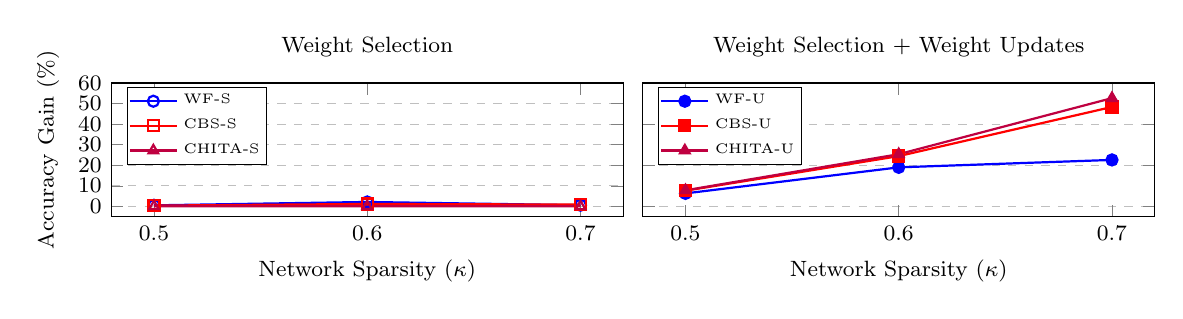
\begin{tikzpicture}

% Selection-Only Subplot
\begin{axis}[
    name=plot1,
    width=6.5cm,
    height=0.14\textwidth,
    scale only axis,
    xlabel={Network Sparsity (\(\kappa\))},
    ylabel={Accuracy Gain (\%)},
    xmin=0.48, xmax=0.72,
    ymin=-5, ymax=60,
    xtick={0.5,0.6,0.7},
    ytick={0,10,20,30,40,50,60},
    ymajorgrids=true,
    grid style=dashed,
    legend pos=north west,
    legend style={font=\tiny, cells={anchor=west}, inner sep=0.5pt},
    tick label style={font=\footnotesize},
    label style={font=\footnotesize},
    title={\footnotesize Weight Selection}
]

% WF-S gain over MP
\addplot[color=blue, mark=o, solid, thick] coordinates {
    (0.5, 0.49)
    (0.6, 2.13)
    (0.7, 0.55)
};
\addlegendentry{WF-S}

% CBS-S gain over MP
\addplot[color=red, mark=square, solid, thick] coordinates {
    (0.5, 0.35)
    (0.6, 1.16)
    (0.7, 0.85)
};
\addlegendentry{CBS-S}

% CHITA-S gain over MP
\addplot[color=purple, mark=triangle, solid, thick] coordinates {
    (0.5, 0.01)
    (0.6, 0.04)
    (0.7, 0.00)
};
\addlegendentry{CHITA-S}

\end{axis}

% Weight Updates Subplot
\begin{axis}[
    name=plot2,
    at={(plot1.east)},
    anchor=west,
    xshift=0.25cm,
    width=6.5cm,
    height=0.14\textwidth,
    scale only axis,
    xlabel={Network Sparsity (\(\kappa\))},
    xmin=0.48, xmax=0.72,
    ymin=-5, ymax=60,
    xtick={0.5,0.6,0.7},
    yticklabels={,,},
    ymajorgrids=true,
    grid style=dashed,
    legend pos=north west,
    legend style={font=\tiny, cells={anchor=west}, inner sep=0.5pt},
    tick label style={font=\footnotesize},
    label style={font=\footnotesize},
    title={\footnotesize Weight Selection $+$ Weight Updates}
]

% WF-U gain over MP
\addplot[color=blue, mark=*, solid, thick] coordinates {
    (0.5, 6.3)
    (0.6, 18.96)
    (0.7, 22.58)
};
\addlegendentry{WF-U}

% CBS-U gain over MP
\addplot[color=red, mark=square*, solid, thick] coordinates {
    (0.5, 7.6)
    (0.6, 24.43)
    (0.7, 48.33)
};
\addlegendentry{CBS-U}

% CHITA-U gain over MP
\addplot[color=purple, mark=triangle*, solid, thick] coordinates {
    (0.5, 7.81)
    (0.6, 25.36)
    (0.7, 52.62)
};
\addlegendentry{CHITA-U}

\end{axis}

\end{tikzpicture}
\caption{Comparison of test accuracy gain of impact-based pruning methods over magnitude pruning for a pre-trained MobileNet on ImageNet at different sparsity levels. \textbf{Left:} Selection-only pruning methods. \textbf{Right:} Pruning methods with weight updates show significant performance gains.}
\label{fig:gain_over_mp_split}
\end{figure}


These findings challenge the conventional assumption and leads to a further question:
\textit{If weight selection—whether based on magnitude or loss-aware criteria—plays a minimal role, what fundamentally drives the performance degradation of one-shot pruned networks?}


Our investigation uncovers a new explanation: \textbf{signal collapse}. One-shot pruning alters the flow of activations through the network, progressively reducing their variance in deeper layers. This leads to signal collapse, where activations in the final layers become nearly constant, preventing the network from distinguishing between inputs. As a result, predictions become uniform, severely impairing performance. While accuracy loss due to pruning is conventionally attributed to the removal of critical parameters, our results reveal that signal collapse is the primary driver of degraded performance in pruned networks.


The key insight from our work is that \textbf{signal collapse can be mitigated} and simple methods, such as MP, can surpass the performance of state-of-the-art IP-based methods. Our work \textbf{REFLOW} (\textbf{Re}storing \textbf{F}low of \textbf{Low}-variance signals) mitigates signal collapse without requiring gradient or Hessian-based computations. REFLOW addresses the overlooked bottleneck of signal collapse, demonstrating that high-performing sparse sub-networks inherently exist within the original parameter space identified.



REFLOW achieves substantial accuracy recovery when applied to networks with various neural network architectures pruned with MP. For instance, at 80\% sparsity on ImageNet, ResNet-152 recovers from under 1\% to 68.2\%, and ResNeXt-101 improves from less than 4.1\% to 78.9\%. These results highlight that \textbf{high-quality sparse models} can be obtained by restoring activation flow rather than optimizing weight selection. REFLOW further reveals that high-performing sparse networks inherently exist within the original weights.


\noindent\textbf{Contributions.} This work makes the following key observations and contributions: \begin{enumerate} 
\item 
For the first time, we identify \textbf{signal collapse as the leading cause of accuracy loss in addition to the removal of critical weights,}. 
\item 
\textbf{Signal collapse can be mitigated without updating any trainable weights.} Our work
REFLOW restores activation flow, enabling networks pruned by MP to outperform IP methods \textit{without gradient or Hessian computations}.
\item 
We demonstrate that \textbf{high-performing sparse sub-networks inherently exist in the original parameter space}. Unlike IP methods, which rely on updating unpruned weights to find a solution outside the original parameter space, our approach addresses signal collapse to uncover these sub-networks directly within the original weights. \end{enumerate}
















% \begin{figure}[h]
% \centering
% \begin{tikzpicture}
% % Signal Magnitude Changes Subplot
% \begin{axis}[
%     name=plot1,
%     width=3.1cm,
%     height=0.14\textwidth,
%     scale only axis,
%     xlabel={Layer Index},
%     ylabel={Relative Change (\%)},
%     xmin=1, xmax=27,
%     ymin=-35, ymax=5,
%     xtick={5,10,15,20,25},
%     ytick={-30,-20,-10,0},
%     ymajorgrids=true,
%     grid style=dashed,
%     legend pos=south west,
%     legend style={font=\tiny, cells={anchor=west}, inner sep=0.5pt},
%     tick label style={font=\tiny},
%     label style={font=\tiny},
%     title={\tiny Signal Magnitude}
% ]
% \addplot[color=blue, mark=o, mark size=0.5pt, solid, thick] coordinates {
%     (1,-0.33) (2,0.79) (3,0.99) (4,2.45) (5,3.69) (6,2.23) (7,0) (8,0.60) 
%     (9,0.65) (10,-1.60) (11,-1.96) (12,-2.58) (13,4.35) (14,0.93) (15,-3.26) 
%     (16,2.60) (17,-10.83) (18,2.24) (19,-13.28) (20,0.06) (21,-14.32) 
%     (22,0.84) (23,-10.46) (24,-3.62) (25,-31.99) (26,-14.52) (27,-5.57)
% };
% \addlegendentry{After Pruning}
% \addplot[color=red, mark=square, mark size=0.5pt, solid, thick] coordinates {
%     (1,-0.41) (2,-0.18) (3,-0.33) (4,-0.15) (5,-0.15) (6,0.05) (7,0.33) 
%     (8,-0.14) (9,-0.08) (10,0.42) (11,0.31) (12,-0.25) (13,-0.18) (14,0.38) 
%     (15,-0.05) (16,-0.07) (17,-0.21) (18,-0.14) (19,-0.24) (20,-0.16) 
%     (21,-0.18) (22,-0.16) (23,-0.64) (24,0.36) (25,-1.42) (26,-0.99) (27,2.10)
% };
% \addlegendentry{After AAR}
% \end{axis}

% % Standard Deviation Changes Subplot
% \begin{axis}[
%     name=plot2,
%     at={(plot1.east)},
%     anchor=west,
%     xshift=0.8cm,
%     width=3.1cm,
%     height=0.14\textwidth,
%     scale only axis,
%     xlabel={},
%     xmin=1, xmax=27,
%     ymin=-70, ymax=5,
%     xtick={5,10,15,20,25},
%     ytick={-60,-40,-20,0},
%     ymajorgrids=true,
%     grid style=dashed,
%     legend pos=south west,
%     legend style={font=\tiny, cells={anchor=west}, inner sep=0.5pt},
%     tick label style={font=\tiny},
%     label style={font=\tiny},
%     title={\tiny Standard Deviation}
% ]
% \addplot[color=blue, mark=o, mark size=0.5pt, solid, thick] coordinates {
%     (1,-0.33) (2,-0.23) (3,-0.37) (4,-3.41) (5,-4.19) (6,-1.86) (7,-4.35) 
%     (8,-4.93) (9,-9.09) (10,-9.17) (11,-11.45) (12,-10.81) (13,-15.73) 
%     (14,-10.18) (15,-18.84) (16,-18.95) (17,-28.87) (18,-25.79) (19,-33.84) 
%     (20,-31.09) (21,-37.36) (22,-37.36) (23,-39.67) (24,-56.18) (25,-57.69) 
%     (26,-67.54) (27,-59.80)
% };
% \addlegendentry{After Pruning}
% \addplot[color=red, mark=square, mark size=0.5pt, solid, thick] coordinates {
%     (1,-2.17) (2,-1.05) (3,-0.88) (4,-0.74) (5,-0.32) (6,0.10) (7,0.03) 
%     (8,-0.29) (9,-0.40) (10,0.10) (11,-0.12) (12,-0.59) (13,-0.95) (14,-0.09) 
%     (15,-0.30) (16,-0.07) (17,-0.15) (18,-0.03) (19,-0.09) (20,-0.20) 
%     (21,-0.12) (22,-0.42) (23,-0.39) (24,-0.62) (25,-0.48) (26,-6.47) (27,-0.68)
% };
% \addlegendentry{After AAR}
% \end{axis}
% \end{tikzpicture}
% \caption{Layer-wise activation changes when pruning MobileNet (ImageNet, 80\% sparsity). \textbf{Left:} Activation magnitude degrades progressively after pruning (-32\%), restored by AAR. \textbf{Right:} Standard deviation collapses in deeper layers (-68\%), mitigated by AAR.}
% \label{fig:signal_changes}
% \end{figure}




% \begin{figure}[t]
% \centering
% \begin{tikzpicture}
% \pgfplotsset{
%     compat=1.16,
%     tick label style={font=\scriptsize},
%     label style={font=\scriptsize},
%     title style={font=\scriptsize},
%     legend style={font=\scriptsize}
% }

% \begin{axis}[
%     width=8cm,
%     height=3.5cm,
%     ybar,
%     bar width=5pt,
%     ylabel={\scriptsize Top-1 Acc. (\%)},
%     ylabel near ticks,
%     xlabel={},
%     symbolic x coords={MobileNet,ResNet50,ResNet101,ResNet152,ResNext101,RegNetX},
%     xtick=data,
%     xticklabel style={rotate=30, anchor=east},
%     ymin=0, ymax=100,
%     ymajorgrids=true,
%     grid style=dashed,
%     legend columns = 2,
%     legend style={
%         at={(0.5,1.15)},
%         anchor=south,
%         draw=none,
%         fill=white,
%         fill opacity=0.7,
%         text opacity=1,
%         cells={anchor=west}
%     },
%     nodes near coords,
%     every node near coord/.append style={font=\tiny, black},
% ]

% % After Pruning (blue)
% \addplot+[fill=blue!20, draw=blue!60!black] 
% coordinates {
%     (MobileNet,0.1)
%     (ResNet50,3.3)
%     (ResNet101,4.1)
%     (ResNet152,0.8)
%     (ResNext101,0.4)
%     (RegNetX,1)
% };
% \addlegendentry{After Pruning}

% % After AAR (red)
% \addplot+[fill=red!20, draw=red!60!black] 
% coordinates {
%     (MobileNet,43)
%     (ResNet50,54)
%     (ResNet101,64)
%     (ResNet152,68)
%     (ResNext101,78.8)
%     (RegNetX,73)
% };
% \addlegendentry{After AAR}

% \end{axis}
% \end{tikzpicture}
% \caption{Post-pruning accuracy at 80\% sparsity using one-shot magnitude pruning (blue) and after applying AAR (red) on ImageNet. Magnitude pruning severely degrades accuracy but AAR substantially recovers performance.}
% \label{fig:accuracy_improvement}
% \end{figure}





















